
\newcommand\QEDit{\hspace{6pt}\textit{Q.~E.~D.}\quad}
\newcommand\QEFit{\hspace{6pt}\textit{Q.~E.~F.}\quad}
\newcommand\QEIit{\hspace{6pt}\textit{Q.~E.~I.}\quad}
\newcommand\QEDup{\hspace{6pt}Q.~E.~D.\quad}
\newcommand\QEFup{\hspace{6pt}Q.~E.~F.\quad}
\newcommand\QEIup{\hspace{6pt}Q.~E.~I.\quad}
\newcommand\QEOup{\hspace{6pt}Q.~E.~O.\quad}
\newcounter{wrapwidth}
\newcount \Zw
\newcount \Zh


\newcommand\pngright[4]{
\Zw=#2 \divide \Zw by 10
\Zh=#3 \divide \Zh by 120  \advance\Zh by 1
\setcounter{wrapwidth}{\Zw}
\begin{wrapfigure}[\Zh]{r}{\value{wrapwidth}pt}
\begin{center}
\vspace{#4pt}
\includegraphics*[width=\Zw pt]{images/#1}
\end{center}
\end{wrapfigure}}

\newcommand\propnopage[1]{
\begin{center}{\large #1}\end{center}}

\parindent1em
\chapter{PERICULA}

\noindent\textsc{Case Study: } We will now typeset a section, from Isaac Newton's \textit{Philosophi\ae\  Naturalis Principia Mathematica}. The typeset example is shown below.

\bottomline
\bgroup
\small

\cxset{section align=center,
       section numbering=none}

\section{{SECT}$\cdot$ VIII$\cdot$}

\begin{center}{\textit{De Motu per Fluida propagato.}}\end{center}

\propnopage{Prop.\ XLI\@. Theor.\ XXXI.}

\textit{Pressio non propagatur per Fluidum secundum lineas rectas, nisi
ubi particul{\ae} Fluidi in directum jacent.}

Si jaceant particul{\ae} $a$, $b$, $c$, $d$, $e$ in linea recta, potest quidem
pressio directe

\begin{wrapfigure}[8]{O}[1pt]{0.3\textwidth}
  \vspace{-17pt}
  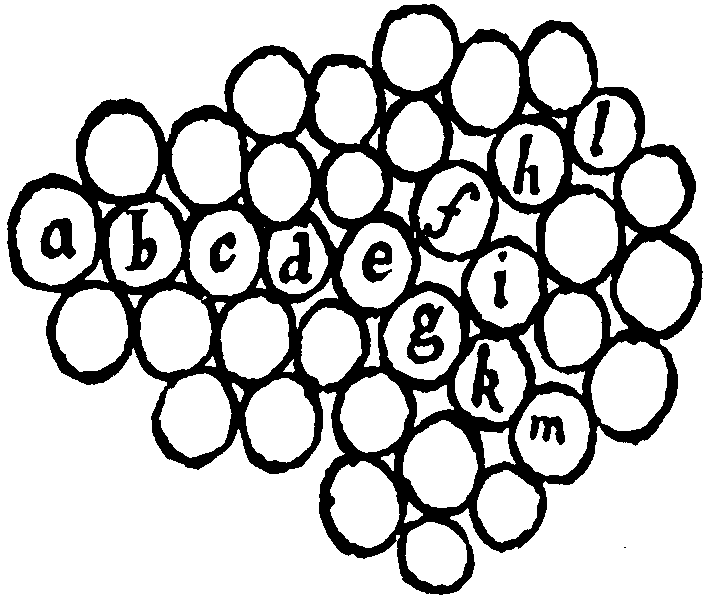
\includegraphics[width=0.27\textwidth]{images/362.png}
\end{wrapfigure}

\noindent propagari  ab $a$ ad $e$; at
particula $e$ urgebit particulas oblique positas
$f$ \& $g$ oblique, \& particul{\ae} ill{\ae} $f$ \& $g$
non sustinebunt pressionem illatam, nisi fulciantur
a particulis ulterioribus $h$ \& $k$;
quatenus autem fulciuntur, premunt particulas
fulcientes; \& h{\ae} non sustinebunt pressionem nisi fulciantur
ab ulterioribus $l$ \& $m$ easque premant, \& sic deinceps in infinitum.
Pressio igitur, quam primum propagatur ad particulas
qu{\ae} non in directum jacent, divaricare incipiet \& oblique propagabitur
in infinitum; \& postquam incipit oblique propagari, si
inciderit in particulas ulteriores, qu{\ae} non in directum jacent, iterum
divaricabit; idque toties, quoties in particulas non accurate
in directum jacentes inciderit. \QEDit

\topline

\vspace*{-\baselineskip}
\captionof{figure}{Example of a typeset page from Principi\ae.}
\egroup
\smallskip
Figure~\ref{fig:principia}, shows a scan of the actual page. We will not reproduce, the fonts and the page geometry exactly, but rather we will attempt to extract and reproduce the typographical rules employed in the printing of the \textit{Principi\ae}.

We begin by typesetting the section number and its heading. The use of roman numbers creates better harmony between the text and the heading
\begin{verbatim}
\sectpage{VIII$\middot$}
\begin{center}{\textit{De Motu per Fluida propagato.}}\end{center}
\end{verbatim}
The proposition and theorem line, has its own command
\begin{verbatim}
\propnopage{Prop.\ XLI\@. Theor.\ XXXI.}
\end{verbatim}

\propnopage{\color{gray}Prop.\ XLI\@. Theor.\ XXXI.}
\vspace*{-37pt}
\propnopage{Prop. XLI. Theor. XXXI.}


Notice the small differences in the spacing with the commands as shown and with the black text, without them. The rest is based on normal \LaTeX\ commands.

\textit{Pressio non propagatur ... particul{\ae}...}

\pngright{362.png}{709}{603}{-24}

Si jaceant particul{\ae} $a$, $b$, $c$, $d$,
$e$ in linea recta, potest quidem
pressio directe propagari ab $a$ ad $e$; at


Remember that it is important to start a new paragraph after the |\pngright| command. The |wrapfig| package works by using |\everypar| to insert the hanging indentation.

\begin{figure}[p]
\centering
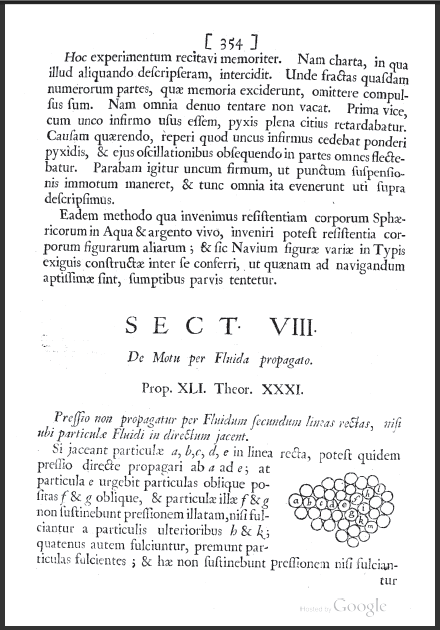
\includegraphics[scale=1]{images/page354}
\caption{Page 354 from Isaac Newton's \textit{Philosophi\ae\  Naturalis Principia Mathematica}. Image was obtained from Google's copy, available at Google Books.}
\label{fig:principia}
\end{figure}
